\section{Attachements}
\subsection{A1 Tiefpassentwurf mit fir()}
\label{cap:A1}
Mit der Matlab Funktion fir() ist ein FIR-Tiefpassfilter zu entwerfen. Als Defaulteinstellung wird als Fensterfunktion das Hamming-Fenster verwendet. Um die geforderten Grenzwerte einzuhalten muss zunächst die Filterordnung mit dem M\_File Kaiser\_Order\_01.m bestimmt werden. Die Ordnung des Filters beträgt damit nach Abschätzung mit der Kaiser-Formel N
= 23. Die Koeffizienten werden mit dem M\_File fir\_1.m gemäß Listing 2 bestimmt. Außerdem wird der Amplitudengang (x=normiert auf Fs/2), das Zeitsignal und der Frequenzgang vor sowie nach dem Filter in einem Diagramm ausgegeben. In den Abbildungen \ref{fig:Attachment_A1_fir_2a_Amplitudengang_PassBand} und \ref{fig:Attachment_A1_fir_2a_Amplitudengang_StopBand} kann gut erkannt werden, das die ripple im Pass- und Stopband eingehalten werden. Die normierten Filterkoeffizienten (normiert auf $\pm$ 1) müssen für die spätere Implementierung in den DSP auf 16-Bit Integer werte angepasst werden. Dazu werden die Koeffizienten mit einem Korrekturfaktor versehen. In Abbildung \ref{lst:fir_2a_matlab} sind die Änderungen von Listing 2 aufgeführt.\\Korrekturwert maximal 1 $\approx$ 32767 $\rightarrow$ 1-Bit Vorzeichen + 15-Bit Wertebereich. 

\begin{equation}
b_{k}(x) = b(x) * 2^{15}-1
\end{equation}

\begin{table}[h]
	\centering
	\begin{tabular}{c | c}
		Parameter	& Werte	\\
		\hline
		Eckfrequenz Durchlassbereich			& $1800~Hz$	\\
		Eckfrequenz Sperrbereich				& $2600~Hz$	\\
		Maximaler Ripple im Durchlassbereich	& $0.5~db$	\\
		Minimale Sperrdämpfung					& $40~db$	\\
		Abtastfrequenz							& $8000~Hz$	\\
	\end{tabular}
\end{table}

\lstinputlisting[style=matlab, caption={fir\_2a.m Matlab-File Auszug - Tiefpassfilter Ordnung 23}, label={lst:fir_2a_matlab}]{Code/fir_2a.m}


\lstinputlisting[style=c, caption={FIR-Filter Koeffizienten Ordnung 23}, label={lst:fir_2a_koeff}]{Code/LP_coeff.h}


\begin{figure}[H]
\centering
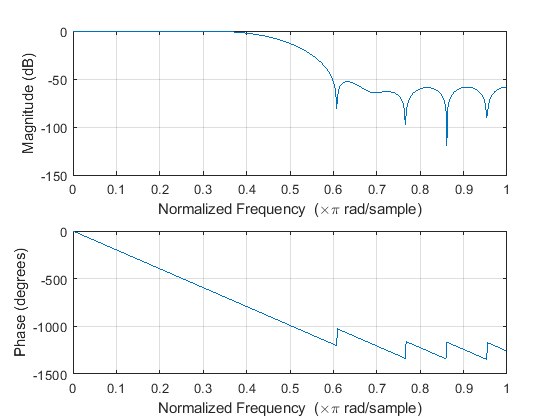
\includegraphics[width=1.0\linewidth]{Bilder/Attachment_A1_fir_2a_Amplitudengang}
\caption{Amplituden und Phasengang - FIR-Filter Tiefpass}
\label{fig:Attachment_A1_fir_2a_Amplitudengang}
\end{figure}


\begin{figure}[H]
\centering
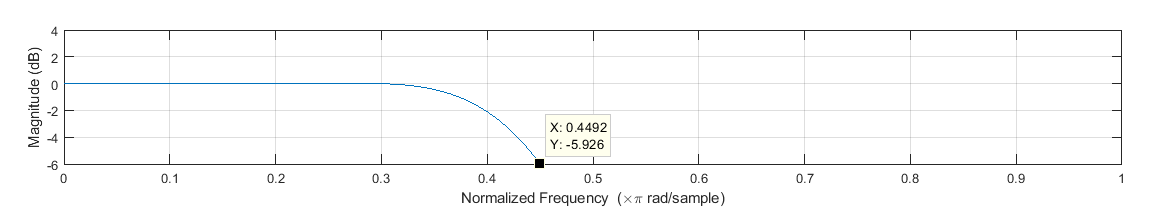
\includegraphics[width=1.0\linewidth]{Bilder/Attachment_A1_fir_2a_Amplitudengang_PassBand}
\caption{Amplitudengang skaliert auf das Passband}
\label{fig:Attachment_A1_fir_2a_Amplitudengang_PassBand}
\end{figure}



\begin{figure}[H]
\centering
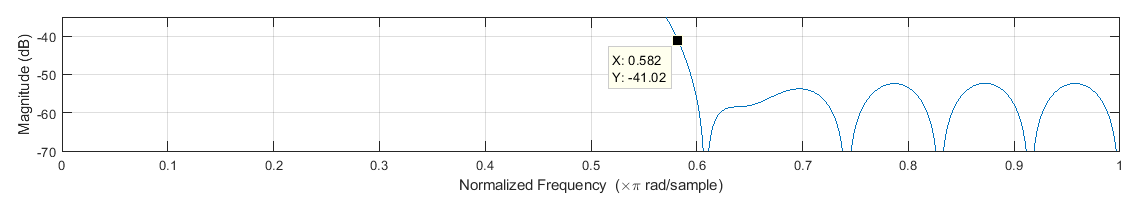
\includegraphics[width=1.0\linewidth]{Bilder/Attachment_A1_fir_2a_Amplitudengang_StopBand}
\caption{Amplitudengang skaliert auf das Stopband}
\label{fig:Attachment_A1_fir_2a_Amplitudengang_StopBand}
\end{figure}

\newpage

\begin{figure}[H]
	\centering
	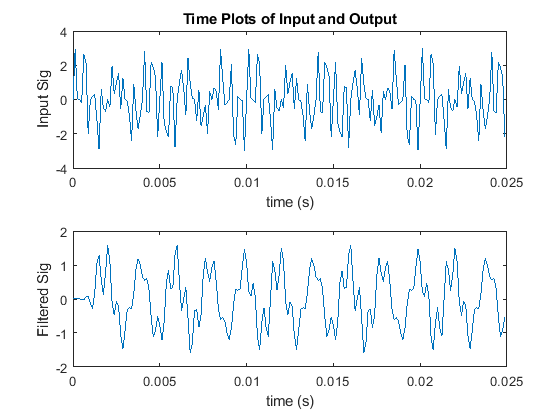
\includegraphics[width=0.75\linewidth]{Bilder/Attachment_A1_fir_2a_Timeplot}
	\caption{Eingangs- und gefiltertes Ausgangszeitsignal  - FIR-Filter Tiefpass}
	\label{fig:Attachment_A1_fir_2a_Timeplot}
	\vspace{-10pt}
\end{figure}

\noindent Im Zeitsignal zeigt sich ebenfalls das Tiefpassverhalten. Es werden hohe Frequenzanteile am Filterausgang ausgefiltert wie in Abbildung \ref{fig:Attachment_A1_fir_2a_Amplitudengang_PassBand} zu erkennen ist.

\begin{figure}[H]
	\centering
	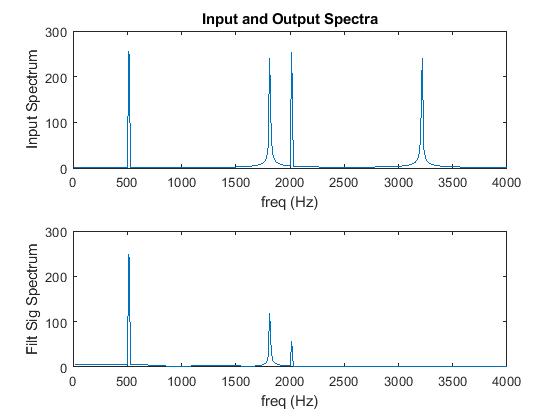
\includegraphics[width=0.75\linewidth]{Bilder/Attachment_A1_fir_2a_Spektrum}
	\caption{Eingangs- gefiltertes Ausgangs Frequenzspektrum}
	\label{fig:Attachment_A1_fir_2a_Spektrum}
	\vspace{-10pt}
\end{figure}

\noindent Das Frequenzspektrum ist in Abbildung \ref{fig:Attachment_A1_fir_2a_Amplitudengang_PassBand} zu erkennen. Es zeigt die Sinussignale bei verschiedenen Frequenzen. Zu erkennen ist das die Signalanteile ab der Durchlassgrenzfrequenz (1800 Hz) schon stark gedämpft werden.

\newpage
\subsection{A2 Tiefpassentwurf mit firpm()}


\noindent Alternativ zur Funktion fir1() soll jetzt die Funktion firpm() verwendet werden um einen FIR-Tiefpassfilter in MATLAB zu entwerfen. In Code-Listing \ref{lst:fir_2b_matlab} sind die Funktionsparameter beschrieben. Die Koeffizienten müssen wie in Kapitel \ref{cap:A1} angepasst werden.

\lstinputlisting[style=matlab, caption={fir\_2b.m Matlab-File Auszug - Tiefpassfilter Ordnung 16/18}, label={lst:fir_2b_matlab}]{Code/fir_2b.m}

\lstinputlisting[style=c, caption={FIR-Filter Koeffizienten Ordnung 16}, label={lst:fir_2b_koeff}]{Code/LP_coeff_firpm_17K.h}

\noindent Mit der Koeffizientenanzahl, die von der Funktion firpmord zurückgeliefert wird kann die geforderte Sperrdämpfung von 40 db nicht eingehalten werden. Der Amplitudengang ist in Abbildung \ref{fig:Attachment_A2_fir_2b_Amplitudengang_17K}, \ref{fig:Attachment_A2_fir_2b_Amplitudengang_PassBand_17K} und \ref{fig:Attachment_A2_fir_2b_Amplitudengang_StopBand_17K} dargestellt. \textbf{Dieser Zustand ist uns erst in der Versuchsnachbereitung aufgefallen, sodass wir alle folgenden Kapitel mit den Filterkoeffizienten der Filterordnung 16 bearbeitet haben}. In den nachfolgenden Kapiteln werden wir diesen Zustand nicht weiter behandeln.\\
Um die geforderten Parameter dennoch einhalten zu können müsste man die Koeffizienten um 2 erhöhen. Dadurch würde es ein Filtersystem 18 Ordnung ergeben und die in den Abbildungen \ref{fig:Attachment_A2_fir_2b_Amplitudengang_19K}, \ref{fig:Attachment_A2_fir_2b_Amplitudengang_PassBand_19K} und \ref{fig:Attachment_A2_fir_2b_Amplitudengang_StopBand_19K} gezeigten Amplitudenverläufe zeigen.\\
Des weiteren ist zu beobachten, dass die Eckfrequenz des Passbereiches sich auf etwa $\approx$ 2.15 kHz verschoben hat. Die Eckfrequenz des Sperrbereiches allerdings fest auf 2.6 kHz geblieben ist.

\begin{figure}[H]
\centering
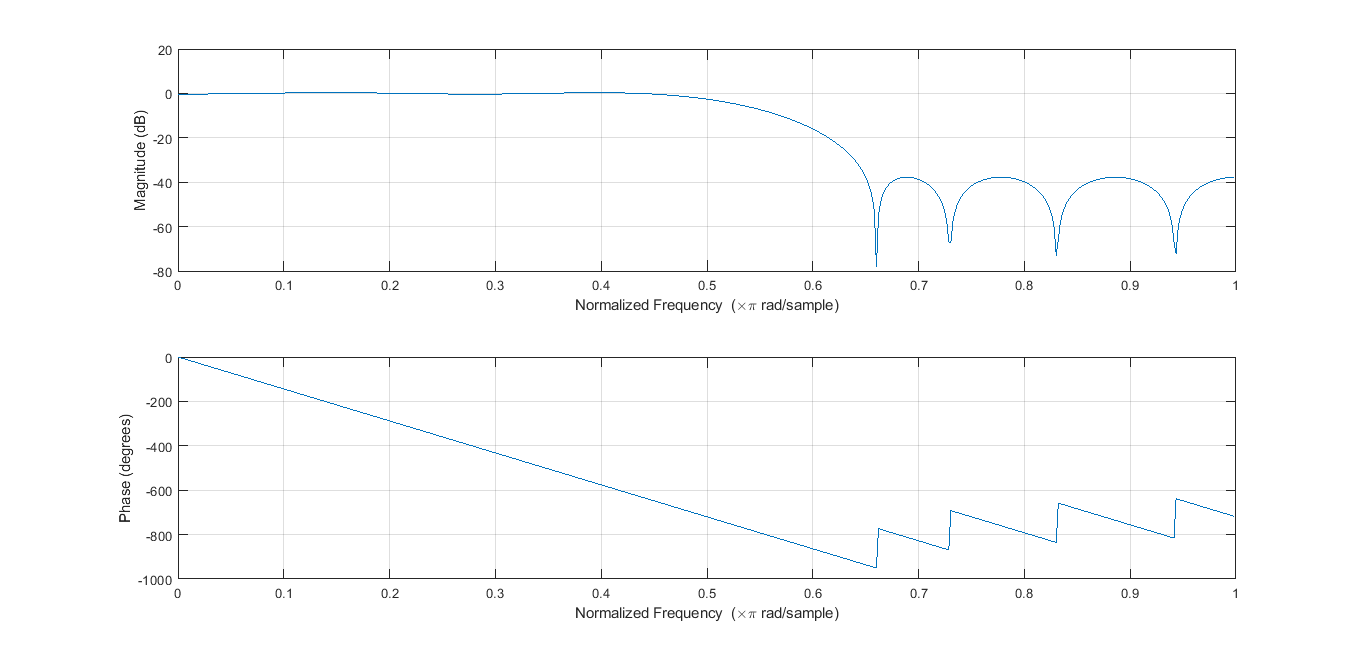
\includegraphics[width=1.0\linewidth]{./Bilder/Attachment_A2_fir_2b_Amplitudengang_17K}
\caption{Amplituden und Phasengang - FIR-Filter Tiefpass - Ordnung: 16}
\label{fig:Attachment_A2_fir_2b_Amplitudengang_17K}
\end{figure}


\begin{figure}[H]
\centering
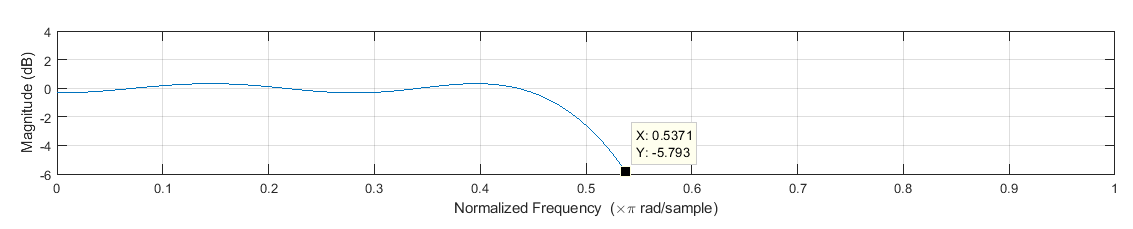
\includegraphics[width=1.0\linewidth]{Bilder/Attachment_A2_fir_2b_Amplitudengang_PassBand_17K}
\caption{Amplitudengang skaliert Passband FIR-Filter Tiefpass - Ordnung: 16}
\label{fig:Attachment_A2_fir_2b_Amplitudengang_PassBand_17K}
\end{figure}

\begin{figure}[H]
\centering
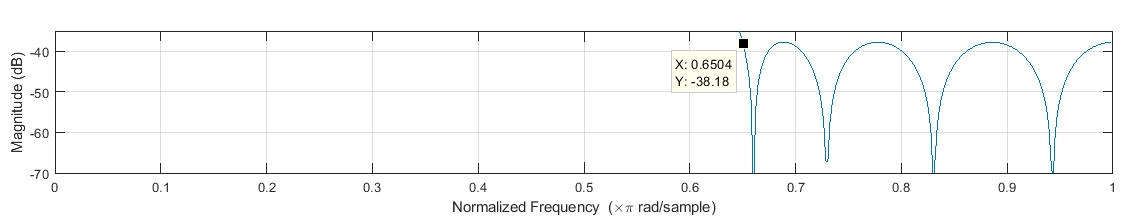
\includegraphics[width=1.0\linewidth]{Bilder/Attachment_A2_fir_2b_Amplitudengang_StopBand_17K}
\caption{Amplitudengang skaliert Stopband FIR-Filter Tiefpass - Ordnung: 16}
\label{fig:Attachment_A2_fir_2b_Amplitudengang_StopBand_17K}
\end{figure}

\newpage


\begin{figure}[H]
	\centering
	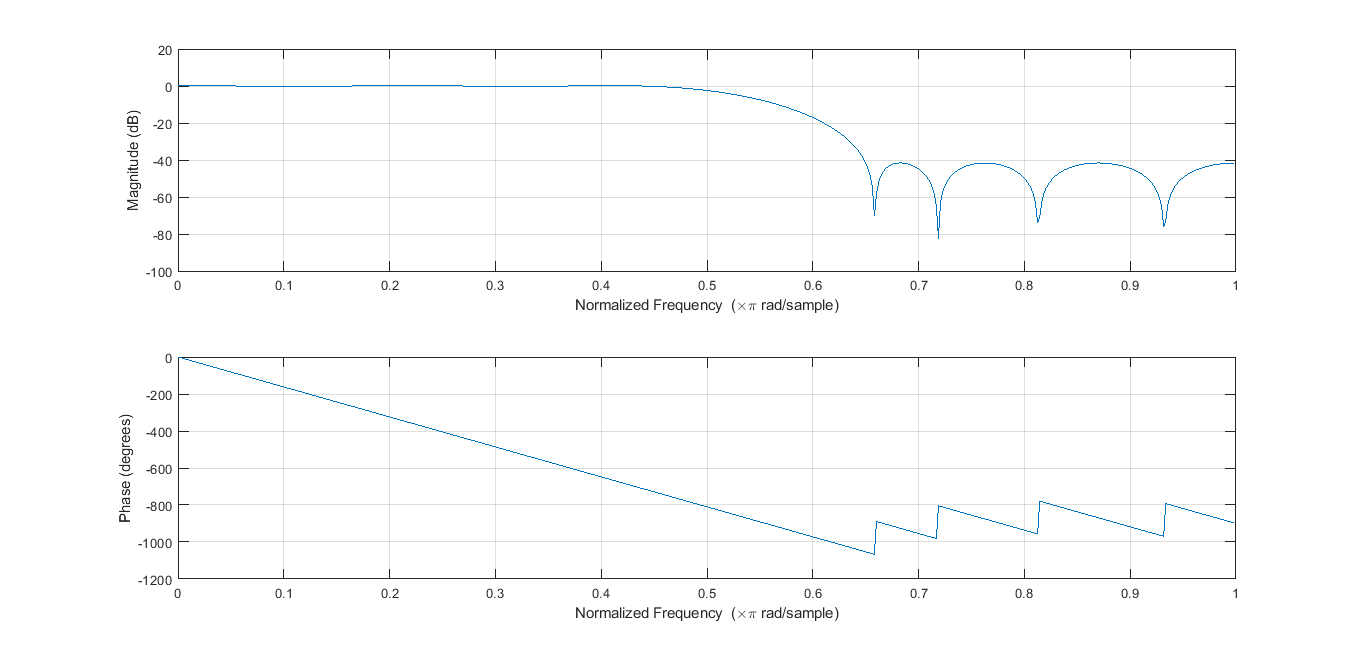
\includegraphics[width=1.0\linewidth]{./Bilder/Attachment_A2_fir_2b_Amplitudengang_19K}
	\caption{Amplituden und Phasengang - FIR-Filter Tiefpass - Ordnung: 18}
	\label{fig:Attachment_A2_fir_2b_Amplitudengang_19K}
\end{figure}


\begin{figure}[H]
	\centering
	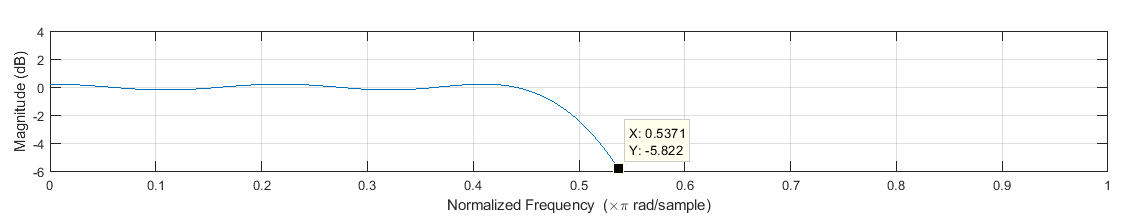
\includegraphics[width=1.0\linewidth]{Bilder/Attachment_A2_fir_2b_Amplitudengang_PassBand_19K}
	\caption{Amplitudengang skaliert Passband FIR-Filter Tiefpass - Ordnung: 18}
	\label{fig:Attachment_A2_fir_2b_Amplitudengang_PassBand_19K}
\end{figure}

\begin{figure}[H]
	\centering
	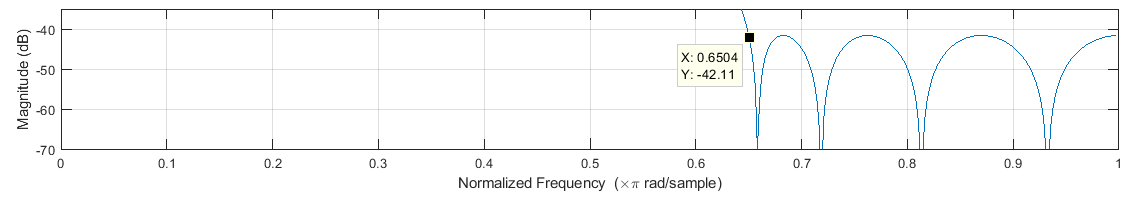
\includegraphics[width=1.0\linewidth]{Bilder/Attachment_A2_fir_2b_Amplitudengang_StopBand_19K}
	\caption{Amplitudengang skaliert Stopband FIR-Filter Tiefpass - Ordnung: 18}
	\label{fig:Attachment_A2_fir_2b_Amplitudengang_StopBand_19K}
\end{figure}

\lstinputlisting[style=c, caption={FIR-Filter Koeffizienten Ordnung 18}, label={lst:fir_2b_koeff}]{Code/LP_coeff_firpm_19K.h}

\newpage


\begin{figure}[H]
\centering
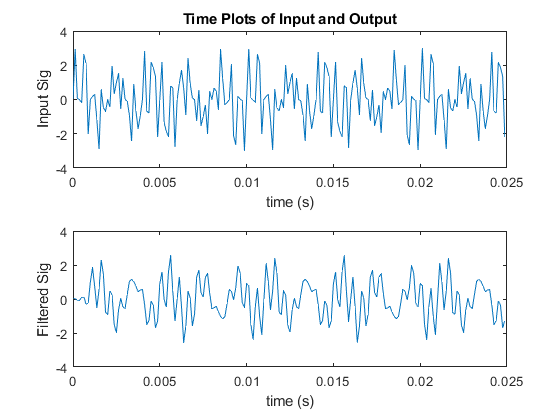
\includegraphics[width=0.85\linewidth]{./Bilder/Attachment_A2_fir_2b_Timeplot}
\caption{Eingangs- und gefiltertes Ausgangszeitsignal  - FIR-Filter Tiefpass}
\label{fig:Attachment_A2_fir_2b_Timeplot}
\end{figure}

\noindent Im Zeitsignal welches Abbildung \ref{fig:Attachment_A2_fir_2b_Timeplot} darstellt sind wie erwartet die hohe Frequenzanteile im Ausgangssignal ausgefiltert.

\begin{figure}[H]
\centering
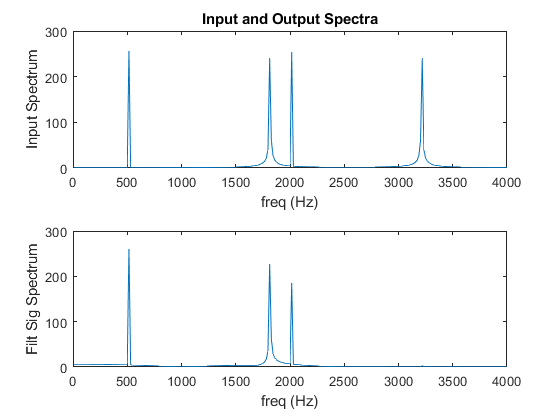
\includegraphics[width=0.85\linewidth]{./Bilder/Attachment_A2_fir_2b_Spektrum}
\caption{Eingangs- gefiltertes Ausgangs Frequenzspektrum}
\label{fig:Attachment_A2_fir_2b_Spektrum}
\end{figure}

\noindent Das Frequenzspektrum zeigt das die Signalanteile die an der Konfigurierten-Eckfrequenz (1800 Hz) des Durchlassbereiches liegen nicht mehr so stark gedämpft werden. Was durch die Erhöhung der Eckfrequenz auf $\approx 2.15 kHz$ verursacht wird.


\noindent Im Vergleich der Matlab Funktionen ist zu erkennen das mit firpm die Filtercharakteristik besser angenähert werden kann. Es wird eine geringer Filterordnung benötigt und bei Gleichen Sperrbereich ist ein größerer Durchlassbereich mit geringerer Dämpfung möglich.

\begin{table}[H]
	\centering
	\begin{tabular}{c | c | c}
						& fir1	&	firpm \\
		\hline	
		Filterordnung	& 23		& 19	\\
		Eckfrequenz Durchlassbereich	& 1.8 kHz	& 2.15 kHz\\ 
		Ripple im Durchlassbereich		& $\approx 0 db$	& $\approx 0.3 db$
	\end{tabular}
\end{table}

\clearpage

\subsection{B Bandpass-Filterentwurf}
\noindent Für den Entwurf eines Bandpassfilters wird das selbe vorgehen wie zur Realisierung eines Tiefpassfilter durchgeführt. In Abbildung \ref{fig:Attachment_B_fir_3_Amplitudengang} sind die Eckfrequenzen des Sperr- und Durchlassbereich markiert. Wie auch schon zuvor beim Tiefpassfilter sind die Eckfrequenzen der Durchlassbereiches nach außen Verschoben, was zu einem Breiteren Durchlassbereich führt. Die Eckfrequenzen des Sperrbereichs sind an den definierten Punkten.

\begin{table}[H]
	\centering
	\begin{tabular}{c | c}
	Parameter	& Werte	\\
	\hline
	Abtastfrequenz		& 8 kHz\\
	Passband			& 0,8 kHz - 2,4 kHz\\
	Transitionband I	& 0,5 kHz - 0,8 kHz\\
	Transitionband II	& 2,4 kHz - 2,7 kHz\\
	Minimale Sperrdämpfung	& 40 db\\
	Maximaler Ripple im Durchlassbereich	& 0,4 db\\
	
	\end{tabular}
\end{table}

\lstinputlisting[style=matlab, caption={fir\_3.m Matlab-File Auszug - Bandpassfilter Ordnung 51}, label={lst:fir_3_matlab}]{Code/fir_3.m}

\lstinputlisting[style=c, caption={FIR-Filter Koeffizienten Ordnung 51}, label={lst:fir_3_koeff}]{Code/BP_coeff.h}

\noindent In Abbildung \ref{fig:Attachment_B_fir_3_Amplitudengang} ist der charakteristische Frequenzgang dargestellt.

\begin{figure}[H]
\centering
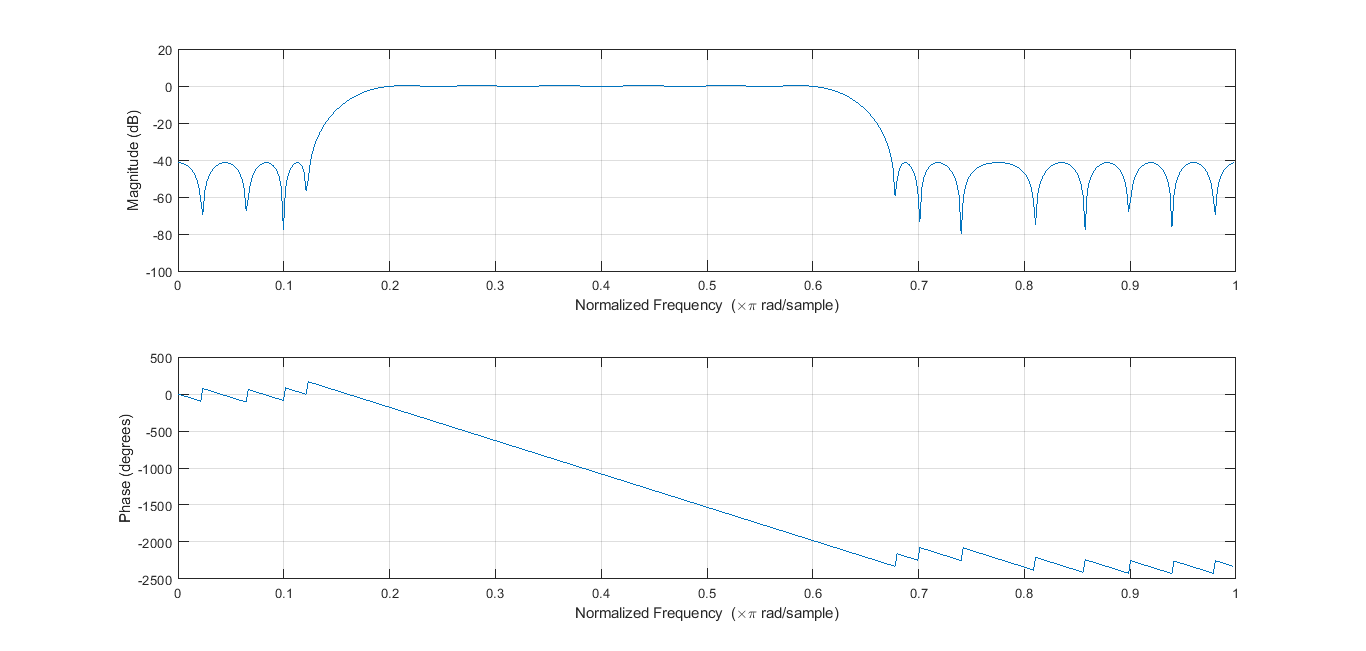
\includegraphics[width=0.9\linewidth]{./Bilder/Attachment_B_fir_3_Amplitudengang}
\caption{Amplituden und Phasengang - FIR-Filter Bandpass}
\label{fig:Attachment_B_fir_3_Amplitudengang}
\end{figure}

\noindent Durch den Bandpassfilter werden die Frequenzanteile im Durchlassbereich nahezu ungedämpft übertragen und die Signalanteile an den beiden Seitensperrbereichen ausgefiltert.

\begin{figure}[H]
\centering
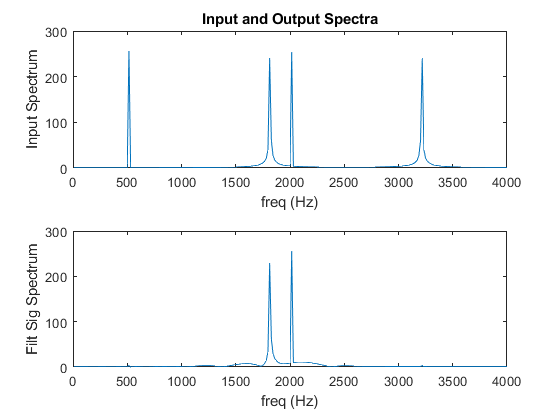
\includegraphics[width=1.0\linewidth]{./Bilder/Attachment_B_fir_3_Spektrum}
\caption{Eingangs- gefiltertes Ausgangs Frequenzspektrum}
\label{fig:Attachment_B_fir_3_Spektrum}
\end{figure}


\begin{figure}[H]
\centering
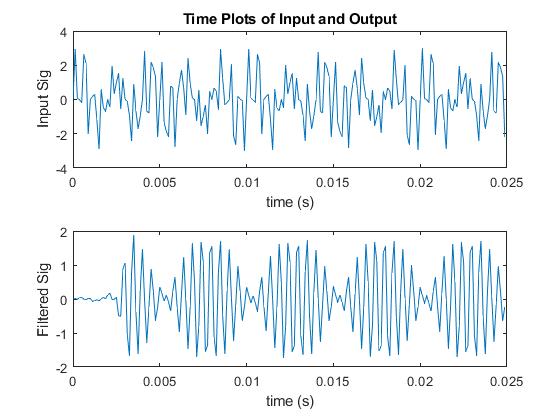
\includegraphics[width=1.0\linewidth]{./Bilder/Attachment_B_fir_3_Timeplot}
\caption{Eingangs- und gefiltertes Ausgangszeitsignal  - FIR-Filter Bandpass}
\label{fig:Attachment_B_fir_3_Timeplot}
\end{figure}

\newpage

\subsection{C1 Analoge Übertragungscharakteristik des DSK Boards}
\noindent Zu Beginn dieses Laborversuchs wurde ein Projekt zu Eingabe sowie anschließenden Ausgabe dieser eingelesenen Werte realisiert, um den Frequenzgang des DSK-Boards zu bestimmen. Im UVP Analyzer wurde ein Messung mit Frequenzsweep bis 8kHz durchgeführt.

\begin{figure}[h]
	\centering
	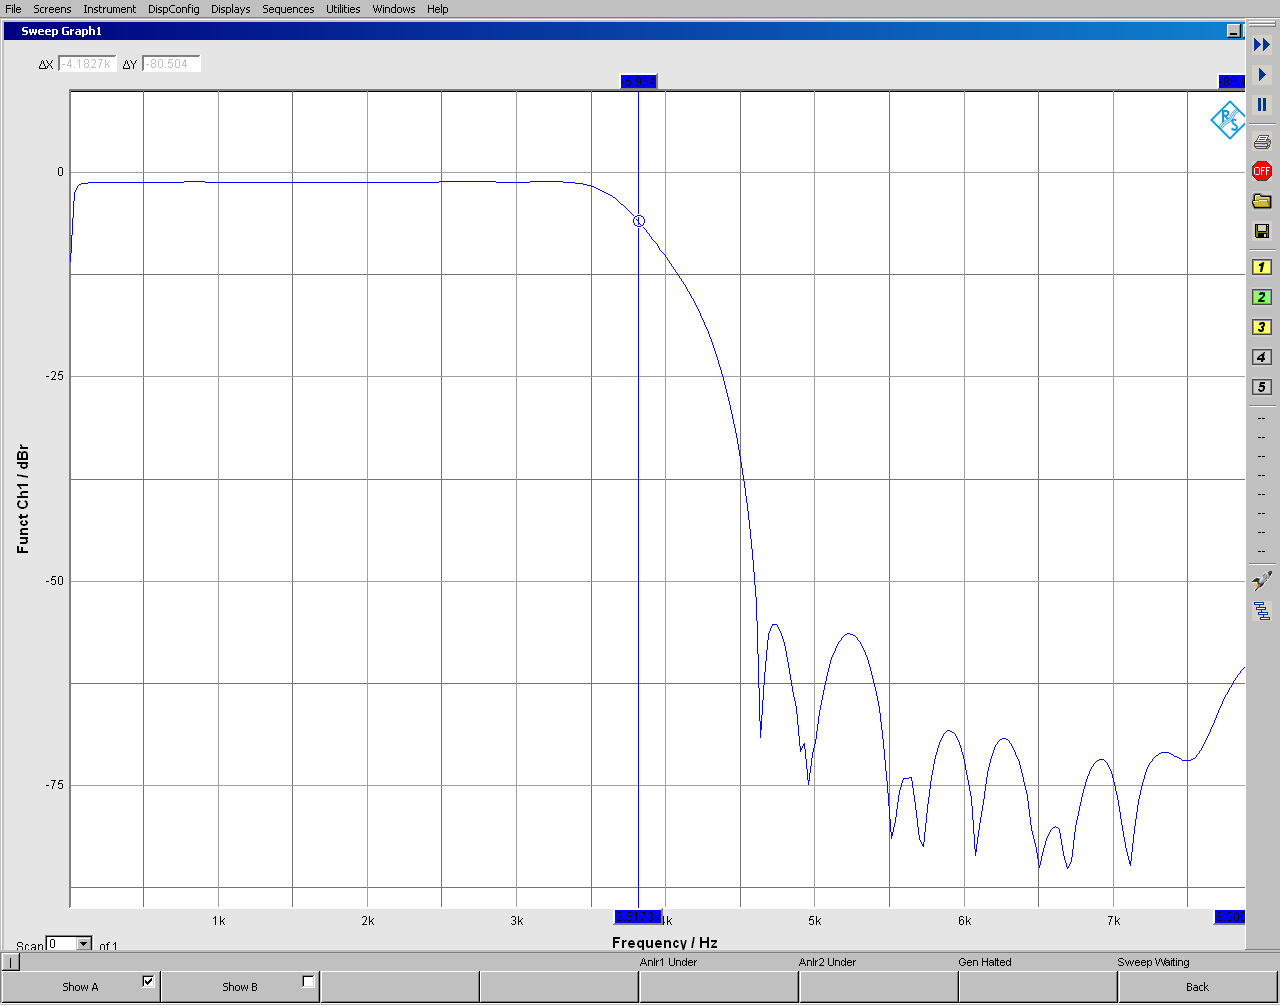
\includegraphics[width=1.0\linewidth]{Bilder/Attachment_C1_DSK_Frequenzgang}
	\caption{Frequenzgang des DSK-Boards}
	\label{fig:Attachment_C1_DSK_Frequenzgang}
\end{figure}

\noindent Wir können ganz klar Tiefpassverhalten des DSK-Boards erkennen. Dies ist für die nächsten Messungen zu berücksichtigen.

\clearpage

\subsection{C2 Echtzeit-Festkomma-Impementierung des FIR-Filters}
\noindent Alle Projekteinstellungen sowie -konfigurationen wurden nach Laboranleitung durchgeführt.\\
\noindent Folgende Änderungen wurden durch uns in fir\_a.c ergänzt: \\
\lstinputlisting[style=c, caption={fir\_a.c C-File Auszug - ISR Tiefpass FIR}, label={lst:fir_a_ISRTP}]{Code/fir_a.c}
\noindent Diese Implementierung in der for-Schleife ab Zeile 18 sowie die anschließende Überschreibung des Wertes (32 Bit auf 16 Bit) nach Beendigung der for-Schleife ist vorteilhaft bezüglich des Rauschverhaltens/der Genauigkeit, da in der erwähnten for-Schleife mit 32 Bit zugunsten der Genauigkeit gerechnet wird. Hierbei treten nur sehr geringe Rundungsfehler auf. Dieser Wert wird dann erst nach der Berechnung auf 16 Bit gecastet. Somit rechnet man so lange wie möglich mit einer hohen Genauigkeit, ohne allzu große Rundungsfehler zu produzieren.

\clearpage

\begin{figure}[h]
	\centering
	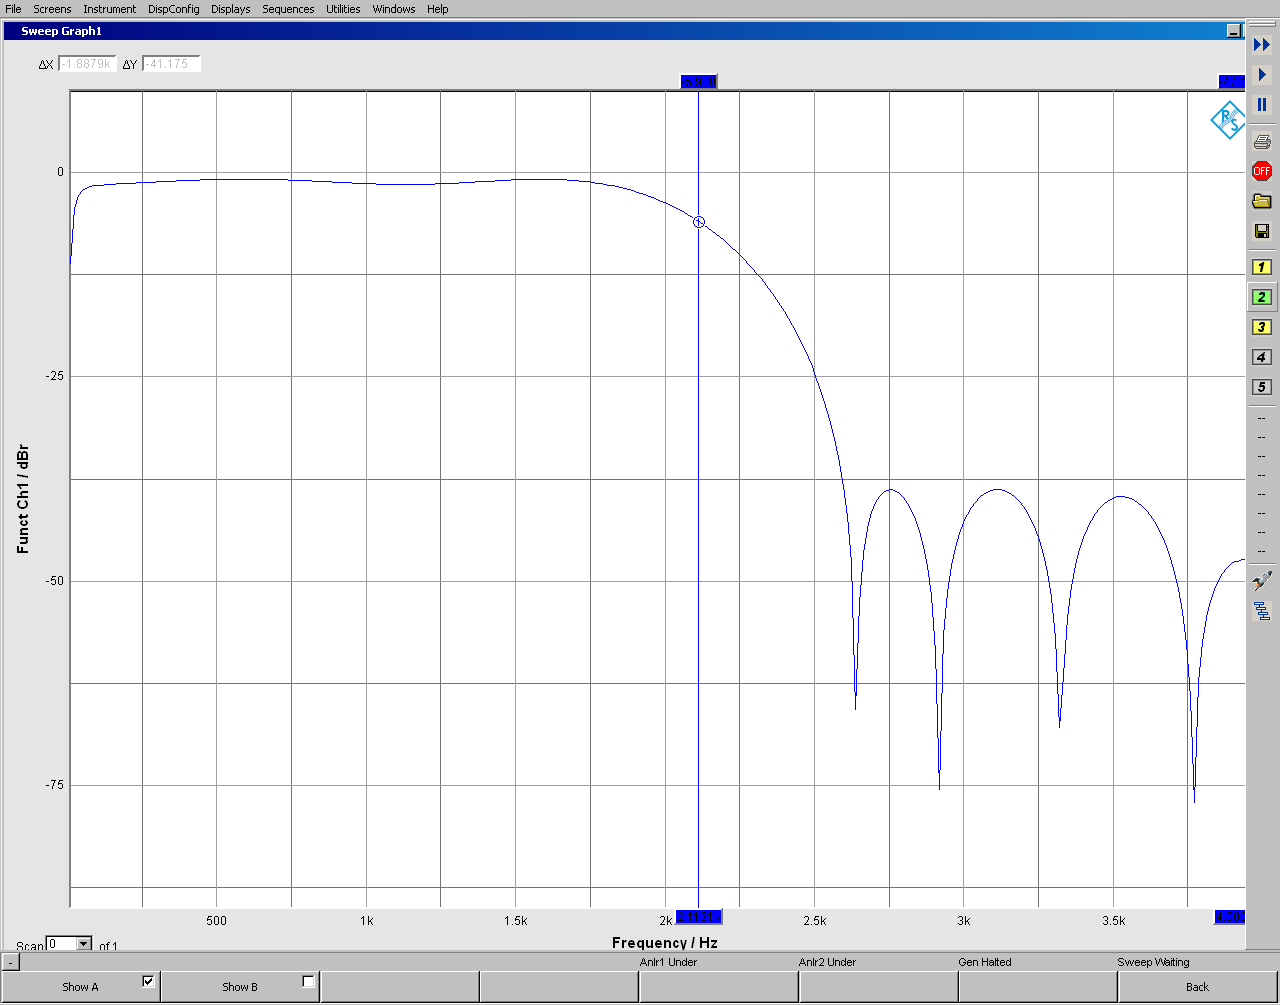
\includegraphics[width=1\linewidth]{Bilder/Attachment_C2_TP_Fg}
	\caption{Messung: Frequenzgang des Tiefpasses mit einem 4kHz Frequenzsweep}
	\label{fig:Attachment_C2_TP_Fg}
\end{figure}

\subsection{C3 Vergleich des Amplitudenganges vom FIR-Filter Matlab - DSK Board}
\noindent Bei der Beurteilung des Amplitudenganges des FIR-Filters muss stets ebenso der Amplitudengang des DSK-Boards berücksichtigt werden. Wie auf Abbildung \ref{fig:Attachment_C1_DSK_Frequenzgang} zu sehen, werden Frequenzen ab 3.5 kHz erst wenig, dann ab $f_g \approx 3.85kHz$) aufgrund des vorgeschalteten Tiefpassfilters (Anti-Aliasingfilter) stärker gedämpft. Mit Berücksichtigung dieser Information fällt beim Frequenzgang des FIR-TP-Filter (Abb. \ref{fig:Attachment_C2_TP_Fg}) auf, dass die letzte Nebenkeule stärker gedämpft wird als die restlichen vorangegangen Nebenkeulen. Dies geschieht, da bei einer Startfrequenz von $\approx3.8kHz$ der letzten sichtbaren Nebenkeule das Anti-Aliasingfilter des DSK-Boards einen entscheidenden  Einfluss bekommt. Dieses Eingangsfilter dämpft bei dieser Frequenz von $\approx3.8kHz$ bereits um fast 6dB. Die Frequenzen $<3.8kHz$ befinden sich im Durchgangsbereich des Eingangsfilters. Diese ermittelte Grenzfrequenz ist durch die Wahl unserer internen Abtastfrequenz von 8kHz bedingt.

\clearpage

\subsection{D Profiling FIR-ISR}
\noindent Ein Profiling der FIR-ISR wurde durchgeführt. Hierbei wurden die vergangen Takte gezählt die benötigt werden, um die ISR vom Eintreten bis zur Beendigung dieser durchzulaufen. Der Inhalt der ISR war bei dieser Messung in die Main (vor Freigabe jeglicher Interrupts) einzufügen. Es wurden eine Anzahl von 1359 Takten bei einer Taktfrequenz von 225Mhz gemessen.

\begin{figure}[h]
	\centering
	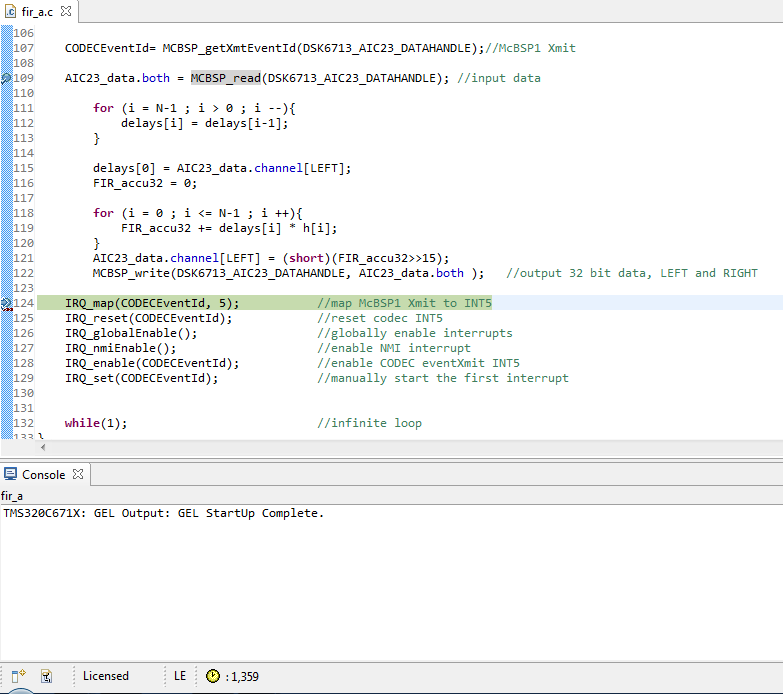
\includegraphics[width=0.9\linewidth]{Bilder/Attachment_D_Profiling}
	\caption{Durchführen des Profilings der FIR-ISR}
	\label{fig:Attachment_D_Profiling}
\end{figure}

\noindent Die maximal erlaubte Abtastfrequenz für dieses FIR-Filter, sodass der nächste Abtastwert noch korrekt eingelesen wird und kein Aliasing entsteht, berechnet sich folgendermaßen:\\

\begin{alignat}{1}
t_{Takt} &= \frac{1}{225Mhz} = 4.5ns \\
t_{ISR}  &= 1359 \cdot 4.5ns = 6.04\mu s \\
\rightarrow f_{max} &= \frac{1}{t_{ISR}} = 165 kHz
\end{alignat}

\clearpage

\subsection{E Tiefpasstransformation mit $h_{TP} \rightarrow h_{HP}$ (Substitution: z = -z)}
\noindent
Aus dem Tiefpassfilter soll mittels Frequenztransformation ein Hochpass implementiert werden. Die Grundidee ist in Abbildung 
\ref{fig:tiefpass_hochpass} schematisch dargestellt.

\begin{figure}[H]
\centering
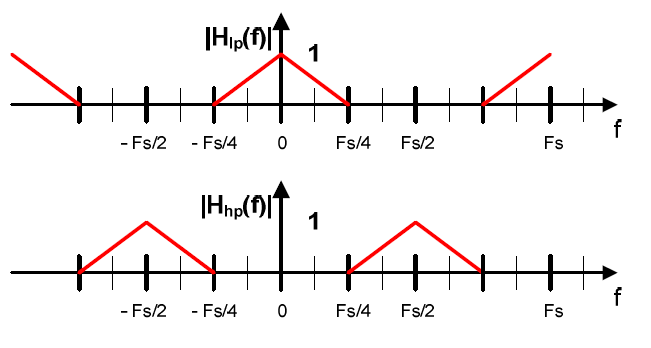
\includegraphics[width=0.7\linewidth]{./Bilder/tiefpass_hochpass}
\caption{Spektrum Tiefpass und Hochpass}
\label{fig:tiefpass_hochpass}
\end{figure}

\noindent Vergleicht man das Spektrum der beiden Filter so ist zu erkennen das der Hochpass nur eine Verschiebung um $\frac{F_{S}}{2} = \pi$ des Tiefpassfilter darstellt und umgekehrt. Mathematisch lässt sich das mit dem Verschiebungssatz beschreiben: $H_{HP}(\omega) = H_{TP}(\omega-\pi)$

\begin{alignat}{1}
H_{TP}(e^{j\omega})&= \sum_{k=0}^{N-1} h_{k_{TP}} \cdot e^{-j\omega k} \rightarrow H_{HP} = H_{TP}(\omega-\pi)= \sum_{k=0}^{N-1} h_{k_{TP}} \cdot e^{-j(\omega-\pi) k} \\
H_{HP}(e^{j\omega})&= \sum_{k=0}^{N-1} h_{k_{TP}} \cdot e^{j\pi k} \cdot e^{-j \omega k}
\end{alignat}

\noindent Im Z-Bereich ergeben sich folgende Zusammenhänge.

\begin{equation}
H_{TP}(z)= \sum_{n=0}^{N-1} b_{n} z^{-n} \rightarrow H_{HP} = H_{TP}(-z)= \sum_{n=0}^{N-1} b_{n} (-z)^{-n} = \sum_{n=0}^{N-1} b_{n} (-1)^n(z)^{-n}
\end{equation}
Daraus lässt sich erkennen das einen Transformation zwischen  Hoch- und Tiefpass lediglich über das Vorzeichen der ungeraden Koeffizienten-Indizes herzuleiten ist. Die Koeffizienten sind im folgenden Listing aufgeführt.

\newpage

\lstinputlisting[style=c, caption={FIR-Filter Koeffizienten Tiefpass \& Hochpass}, label={lst:fir_coeff_TP_HP}]{Code/coeff_firpm_attachement_e.h}

\begin{figure}[H]
\centering
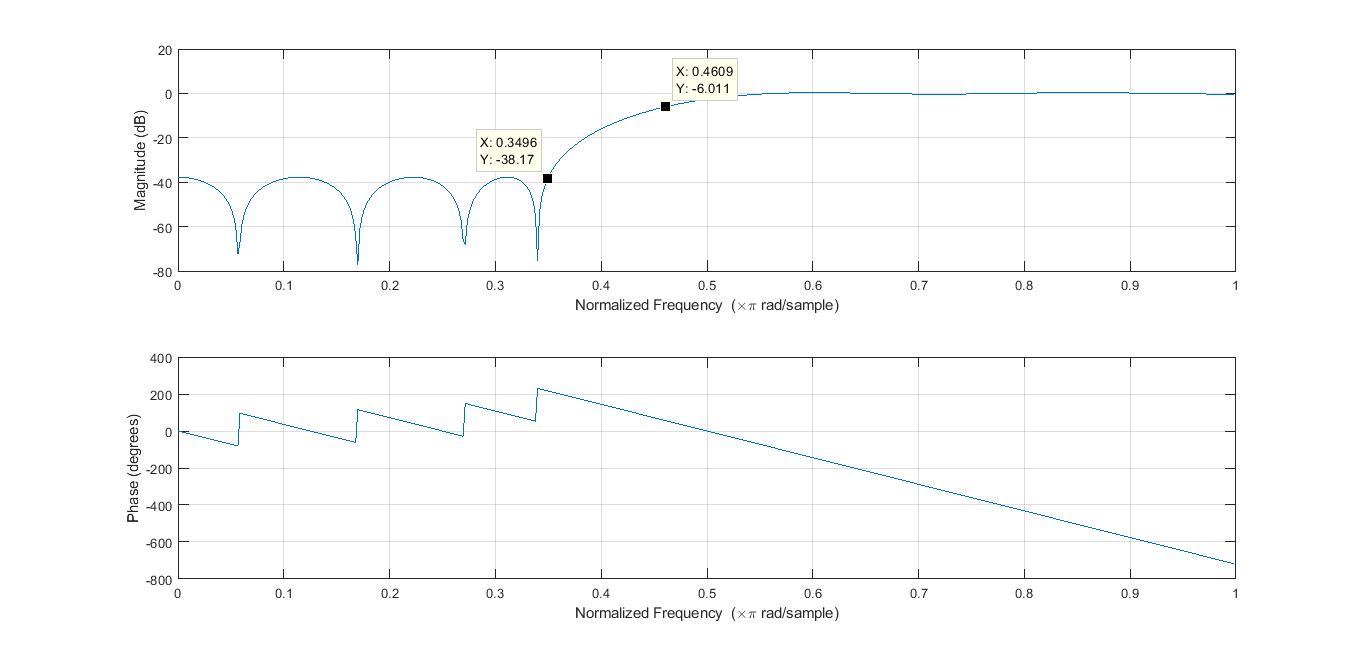
\includegraphics[width=1.0\linewidth]{Bilder/Attachment_E_fir_4_Amplitudengang}
\caption{Amplitudengang Weichenfilter}
\label{fig:Attachment_E_fir_4_Amplitudengang}
\end{figure}

\noindent Der gezeigt Amplitudengang des Weichenfilters in Abbildung \ref{fig:Attachment_E_fir_4_Amplitudengang} hat seine Eckfrequenzen im Sperrbereich bei $f_{g_{Sperr}} \approx 1,4 kHz$ und im Passbereich bei $f_{g_{Sperr}} \approx 1,84 kHz$


\clearpage
\subsection{F Weichenfilter Amplitudengang Hoch- und Tiefpass}
\noindent \noindent Alle Projekteinstellungen sowie -konfigurationen wurden nach Laboranleitung durchgeführt. \\
\noindent Folgende Änderungen wurden durch uns in fir\_b.c ergänzt: \\
\lstinputlisting[style=c, caption={fir\_b.c C-File Auszug - Weichenfilter}, label={lst:fir_b_ISRHPTP}]{Code/fir_b.c}

\clearpage

\noindent Nach der Implementierung wurde eine Messung mit einem Frequenzsweep von 4kHz durchgeführt:

\begin{figure}[h]
	\centering
	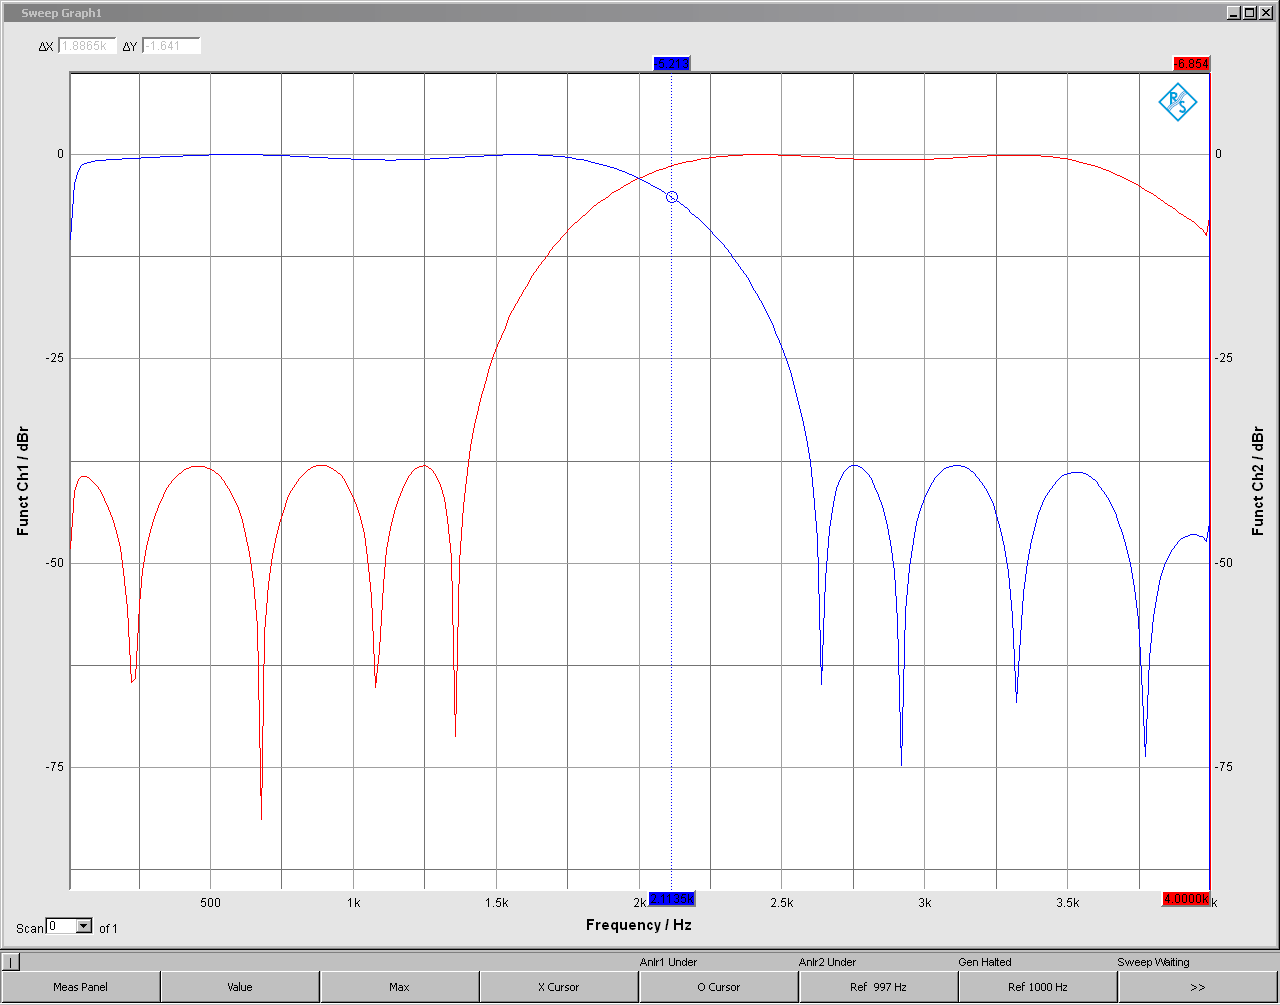
\includegraphics[width=1\linewidth]{Bilder/Attachment_F_HPTP}
	\caption{Messung: Frequenzgang des Weichenfilters mit einem 4kHz Frequenzsweep}
	\label{fig:Attachment_F_HPTP}
\end{figure}

\noindent Die beiden Amplitudengänge entsprechen unseren Erwartungen. Der Hochpass ist der gespiegelte Verlauf des Tiefpasses. Beide Sperrbereiche zeigen die gleiche Ripple-Charakteristik und Sperrdämpfung.
Im Durchlassbereich ist dies nicht so (siehe Abknicken des Durchlassbereiches des Hochpasses ab 3.5kHz),da ab 3.5kHz der Amplitudengang des DSK-Boards Einfluss nimmt. \\
\noindent Zur Programmierung der MAC-Schleife: \\
\noindent Als Grundlage diente die MAC-Schleife des FIR-Tiefpassfilters. Alle benötigten Elemente und Variablen wurden einmal für die Berechnung des FIR-Tiefpasses sowie einmal für die Berechnung des FIR-Hochpasses angelegt. Die Multiply-Accumulate-Operation für den Tiefpass blieb erhalten, lediglich eine zweite Zeile für die Multiply-Accumulate-Operation des Hochpasses wurde innerhalb dieser Schleife hinzugefügt.

\clearpage

\subsection{G Tiefpasstransformation mit $h_{TP} \rightarrow h_{HP}$ (Änderung des mittleren Koeffizienten)}
\noindent Nun sollte nur das FIR-Tiefpassfilter gemessen werden. Dem mittlere Koeffizienten (Anzahl d. Koeffizienten muss folglich ungerade sein) wurde der Wert 32767 im Watch-Window des CCS subtrahiert.\\
Folgende Abbildung zeigt die Messung mit einem Frequenzsweep von 4kHz des Analyzers:\\

\begin{figure}[h]
	\centering
	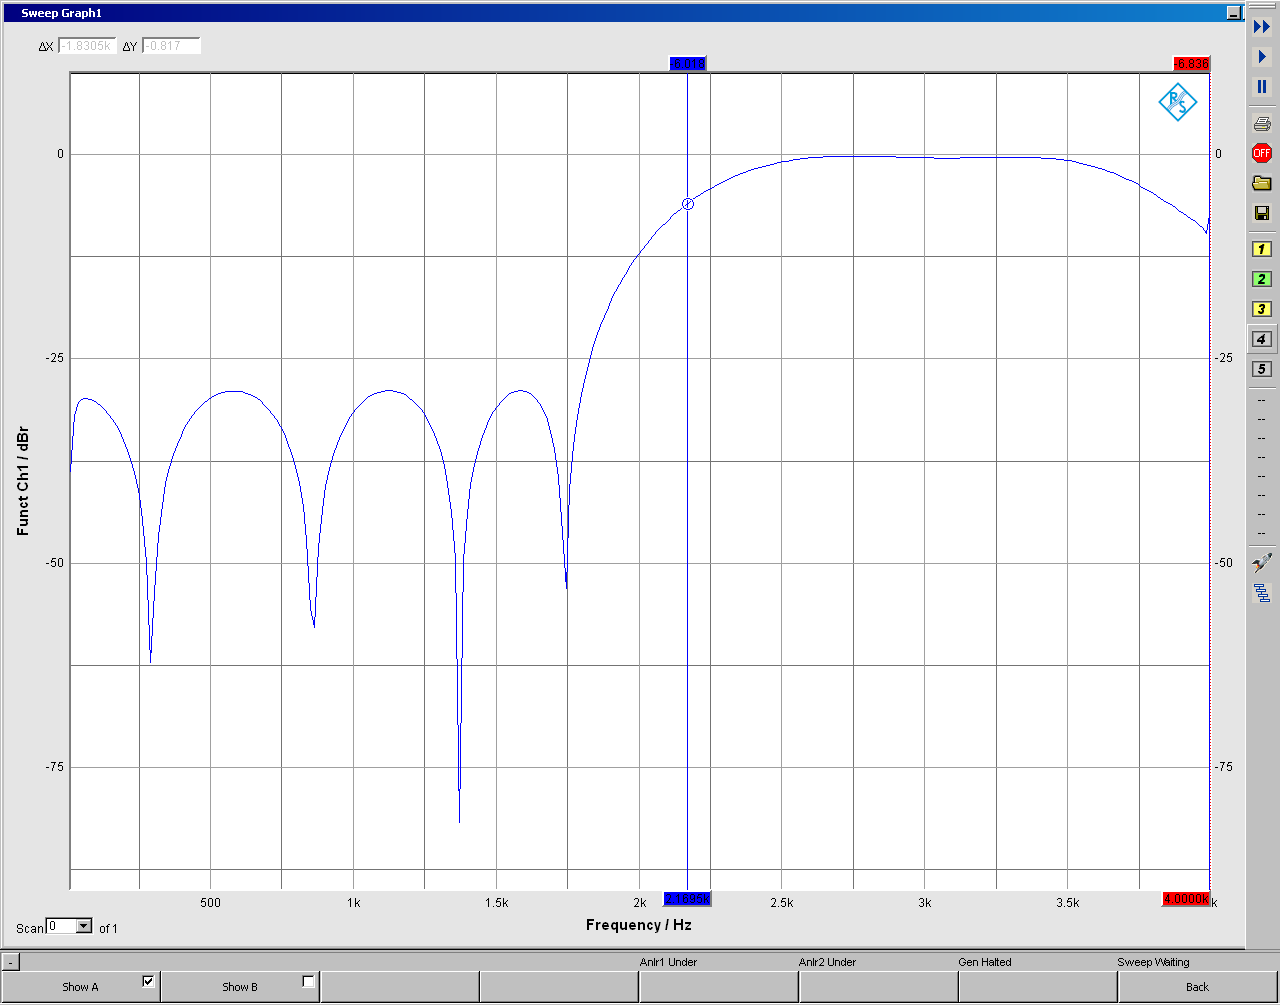
\includegraphics[width=1\linewidth]{Bilder/Attachment_G_1-TP}
	\caption{Messung: Frequenzgang des FIR-Tiefpasses (Änderung des mittleren Koeffizienten) mit einem 4kHz Frequenzsweep}
	\label{fig:Attachment_G_1-TP}
\end{figure}

 
